\section{Approach}
\label{sec:approach}

Here we first give a short outline of our approach and then
  provide a more detailed description of the individual steps.

\subsection{Outline of the approach}

We start by assuming that we are given an identity relation $\approx$.
We will then reinterpret this relation as an indiscernibility relation
  relative to different sets of predicates.
Pairs that have the same indiscernibility predicates
  are simi-discernible, i.e. they discern resources
  based on the same criteria.
Simi-discernibility is an equivalence relation $\equiv_{\indp_{\approx}}$
  which partitions all pairs and thus also the identity relation $\approx$.
The members of the indiscernibility partition
  have a certain overlap with the original identity relation.
The overlap between an indiscernibility subset and the identity relation
  is called an \emph{identity subrelation}.
Each identity subrelation is characterized in terms of predicates
  from the domain vocabulary.
Different forms of identity can therefore be distinguished
  and meaningfully described.
Based on whether there is a complete or a partial overlap
  between the simi-discernible partition members and
  the identity subrelations,
  these partition members belong either to the lower ($\lowerapprox$)
  or to the higher approximation ($\higherapprox$) of $\approx$.
Besides setting a lower and a higher bound to the identity relation,
  we can also calculate the precision for each identity subrelation.

\subsection{Preliminaries}
\label{sec:preliminaries}

%TODO 'reosurce'->'object'
%TODO explain that 'objects' are not 'object terms'
%     and are not even (always) denoted by object terms.

$G$ denotes an RDF graph. It consists of a set of ground binary
predicates $p(s,o)$, called ``triples'' in Semantic Web jargon, and often
written as $\triple{s}{p}{o}$. These triples form a graph with all
subjects $s$ and objects $o$ as nodes, and 
each assertion $p(s,o)$ corresponding to a directed edge labelled $p$
between $s$ and $o$. 

We assume that graphs are always closed under
  RDFS and OWL-DL entailment
  (see section \ref{sec:implementation} for details).

We identify subsets of RDF terms based on
  their positional occurrence in triples in $G$:
  $S_G$, $P_G$, and $O_G$ denote the subject, predicate and object terms
  in $G$ respectively.

The interpretation $I$ maps RDF terms onto resources,
  and triples onto truth values.
The extension function $Ext$ maps resources onto pairs of resources.
$I(\triple{s}{p}{o})$ is true iff
  $\pair{I(s)}{I(o)} \in Ext(I(p))$ \cite{Hayes2004}.

A note on terminology: Our use of the word `property' does not coincide
  with the notion of an RDF property, but is closer to the notion
  of a FOL property. Our use of the word `relation' will be close to
  both the notion of a FOL relation and the notion of an RDF property.
  We briefly explain the distinctions.

An RDF property is a resource (i.e., a member of the domain)
  that is the interpretation of
  an RDF term that occurs in the predicate position of a triple.\footnote{
    Notice that we do not use the posibility modality in this formulation.
    Every URI \emph{could} occur in the predicate position of a triple,
      but some URIs are known to denote non-property resources.
  }
As the example above shows, the extension of an RDF property is
  a binary \emph{FOL relation},
  i.e. a subset of the cartesian product of the domain.\footnote{
    In RDF the domain is the set of RDF resources.}

A \emph{FOL property} is a subset of the domain.
The correlate of a FOL property in RDF is a pair that consists of
  a predicate term and an object term (in that order).
The extension of the interpretation of such a pair $\pair{p}{o}$
  is $Ext(I(p))(I(o))$, which is -- indeed -- a set of RDF resources.

In section \ref{sec:path_expressions} we will generalize
  both the concept of a property and the concept of a relation.
Generalized properties will still be similar to FOL properties
  and generalized binary relations will still similar to binary FOL relations,
  but the latter will no longer correspond to a (single) RDF property.

\begin{comment}
$\equivset{x}$ is the equivalence class for $x$
  under equivalence relation $\approx$.
\end{comment}


\subsection{Shared properties and indiscernibility}
\label{sec:indiscernibility}

We assume that we are given an identity relation $\approx$,
  which partitions the subject terms $S_G$ according to
  equation \ref{eq:equivalence_set}.

%\small
\begin{equation}
\label{eq:equivalence_set}
  \equivset{x}
=
  \setdef{
    y \in S_G
  }{
    \equivpair{x}{y}
  }
\end{equation}
%\normalsize

%\subsection{Identity relation -> indiscernibility criteria}

Identity can be defined as the smallest equivalence relation,
  i.e. the most fine-grained partition of $S_G$.
For reasoning purposes, mainly the fact that $\approx$
  is an equivalence relation counts.
As we saw in principle \ref{principle:indiscernibility_of_identicals},
  identity implies indiscernibility with respect to all properties.

We can generalize the notion of indiscernibility,
  by parameterizing the set of properties with respect to which
  indiscernibility is determined.
According to this generalization,
  resources $x$ and $y$ are indiscernible with respect to
  a set of properties $P \subseteq P_G \times O_G$
  iff $\forall_{p \in P}(p(x) \leftrightarrow p(y))$ is the case.

It is important to note that every indiscernibility relation
  is also an equivalence relation (reasoning!),
  although not necessarily the smallest one.
Moreover, every indiscernibility relation defined over the domain $S_G$
  is also an identity relation,
  only over a different domain \cite{Quine1950}.\footnote{
    For instance, the set of properties
      ``has an income of $x$ euro's a month''
      for decimals $x$ do not identify people
      (since two people may have the same income),
      but it does identify income groups.
    }

We now reinterpret the identity relation $\approx$,
  as if it were an indiscernibility relation
  whose set of properties $P$ is implicit.
Based on the identity relation,
  we can make the set of properties explicit
  so that $\approx$ becomes an indiscernibility relation.
Definition \ref{def:indiscernibility_properties} makes
  the properties relative to which terms $x_i$ are indiscernibile
  explicit.

\begin{definition}[Indiscernibility properties]
\label{def:indiscernibility_properties}
\begin{align}
  \indpo_{\approx}(\set{\range{x_1}{x_n}})
=
  \setdef{
    \pair{p}{o} \in P_G \times O_G
  }{\nonumber\\
    \bigwedge_{1 \leq i \leq n}
      \exists p_i \in \equivset{p},
        \exists o_i \in \equivset{o}(
          \triple{x_i}{p_i}{o_i} \in G
        )
% Alternatively, we can place the quantifies outside the conjunction:
%    \exists_{\range{p_1}{p_n} \in \equivset{p}},
%      \exists_{\range{o_1}{o_n} \in \equivset{o}}
%        \bigwedge_{1 \leq i \leq n} \triple{x_i}{p_i}{o_i} \in G
  }\nonumber
\end{align}
\end{definition}

\noindent Notice that in definition \ref{def:indiscernibility_properties}
  we close both the predicate terms $p$ and the object terms $o$
  under identity.
This may be important,
  since ``Berlin'' and ``Berlijn'' (i.e., the Dutch spelling of ``Berlin'')
  may denote identical resources, as may ``lives in'' and ``woont in''
  (i.e., the Dutch spelling of ``lives in'').
When being given data stating that ``Person $a$ lives in Berlin''
  ``Person $b$ woont in Berlijn'', $a = b$, $\text{Berlin} = \text{Berlijn}$,
  and $\text{lives is} = \text{woont in}$,
  we want to identify the permutations of
  $\set{\text{lives in},\text{woont in}}$ and
  $\set{\text{Berlin},\text{Berlijn}}$
  as the indiscernibility properties.

Using definition \ref{def:indiscernibility_properties},
  we can deduce that the indiscernibility properties for
  the identity pair $\pair{\text{Amsterdam}}{\text{Berlin}}$
  would contain (amongst many others) the properties
  ``is a city'', ``has more than 100,000 inhabitants'', and
  ``is located in Europe''.

But we are not only interested in the properties that resources share
  with one other (e.g., being a city, having more than 500,000 inhabitants).
We are also interested in the predicates that a set of resources share.
This amounts to a simple abstraction of
  definition \ref{def:indiscernibility_properties},
  equating the sets of objects (closed under identity)
  and only returning the set of shared RDF predicate terms
  (see definition \ref{def:indiscernibility_predicates}).

\begin{definition}[Indiscernibility predicates]
\label{def:indiscernibility_predicates}
\begin{align}
  \indp_{\approx}(\setrange{x_1}{x_n})
=
  \setdef{
    p \in P_G
  }{
    \exists_{\range{p_1}{p_n} \in \equivset{p}}(\\
        \equivset{
          \setdef{
            o \in O_G
          }{
            \triple{x_1}{p_1}{o}
          }
        }
      =
        \ldots
      =
        \equivset{
          \setdef{
            o \in O_G
          }{
            \triple{x_n}{p_n}{o}
          }
        }
    )
  }\nonumber
\end{align}
\end{definition}

We are also interested in resource pairs that share their sharing properties.
We can thus identify subsets of an identity relation based on differences
  in the sets of predicate path maps relative to which they take resources
  to be \emph{indiscernible} from one another.


We call the predicates that are shared by a set of identical resources $X$
  the indiscenibility criteria for $X$
  (def. \ref{def:indiscernibility_criteria}).

EXAMPLE HERE (PREFERABLY IIMB).

\begin{comment}
Drawing:
<s,p,o1>
<s,p,o2>
<o1,=,o2>
From IIMB data.
\end{comment}

\subsection{Indiscernibility criteria -> identity subrelation}

When we look at the triples that constitute a set of identity relations,
  we see that all identity assertions look the same.
But when we take the properties of those identical resources into account,
  we observe that within a given identity relation there can be different
  subrelations that can be characterized by different sets of properties.

For instance, in the IIMB dataset there are some identical resources that
  share the property \verb|IIMBTBOX:spoken_in|, while other pairs share
  the property \verb|IIMBTBOX:form_of_government|.
The set of pairs of resources that are spoken in the same language may even
  be disjoint from the set of pairs of resources that have the same
  form of government, indicating identity according to different criteria.
In this example, one subset of the identity relation does not discern
  resources that are spoken in the same language, whereas another subset
  of the identity relation does not discern resources that have the same
  form of government.

We say that two resource pairs are indiscernible
  in case both pairs are indiscernible for the same
  $P \subseteq \powerset{P_G}$
  (def. \ref{pair indiscernibility}).

\subsection{Indiscernibility partition -> identity subrelations}

Based on the indiscernibility criteria,
  i.e. the sets of properties that are shared by identical resources,
  we can derive those resource pairs that share
  the same sharing properties.
We can thus identify subsets of an identity relation based on
  differences in the sets of properties relative to which
  the resource pairs that they consist of are
  (in)discernible from one another.
Identity of indiscernibility criteria provides
  another equivalence relation
  ($\approx_{\indp}$, def. \ref{def:indiscernibility_partition}),
  that partitions the identity relation $\approx$ into
  identity subrelations that characterize identity based on different
  indiscernibility criteria.

\begin{definition}[Indiscernibility partition]
\label{def:indiscernibility_partition}
\begin{align}
  \approx_{\indp}
=
  \setdef{
    \pair{\pair{x_1}{x_2}}{\pair{y_1}{y_2}} \in (S_G^2)^2
  }{\\
    \indp_{\approx}(\set{x_1,x_2}) = \indp_{\approx}(\set{y_1,y_2})
  }\nonumber
\end{align}
\end{definition}


\footnote{
  $P$ must be closed under the identity relation, i.e.,
  \begin{equation*}
    cl_{\sim}(P) = \bigcup_{\tuple{\range{p_1}{p_n}} \in P}\nolimits (
      [p_1]_{\sim} \times \ldots \times [p_n]_{\sim}
    )
  \end{equation*}
}

\small
\begin{definition}[Indiscernibility]
\begin{align}
\label{def:resource_indiscernability}
\mathit{IND}(P) \,=\,
  \setdef{
    \pair{x}{y} \in S_G^2
  }{
    \forall_{p \in cl_{\sim}(P)} f_p(x) \approx f_p(y)
  }
\\
\label{pair indiscernibility}
\mathit{IND}(P^*) \,=\,
  \setdef{
    \pair{\pair{x_1}{y_1}}{\pair{x_2}{y_2}} \in (S_G^2)^2
  }{\\
    \forall_{P \in P^*}
        \pair{x_1}{y_1} \in \mathit{IND}(P)
      \leftrightarrow 
        \pair{x_2}{y_2} \in \mathit{IND}(P)
  }\nonumber
\end{align}
\end{definition}
\normalsize

\noindent According to the standard definition,
  identical resources are indiscernible with respect to all properties.
We take a given set of identity pairs and partition it into subsets which
  we can describe as being $cl_{\sim}(P)$-indiscernible,
  for $P \subseteq P_G^n$.

Fig. 1 shows an example
  of a discernibility partitioning for a given identity relation.

\begin{comment}
\begin{figure*}
\label{fig:iimb_example}
\centering
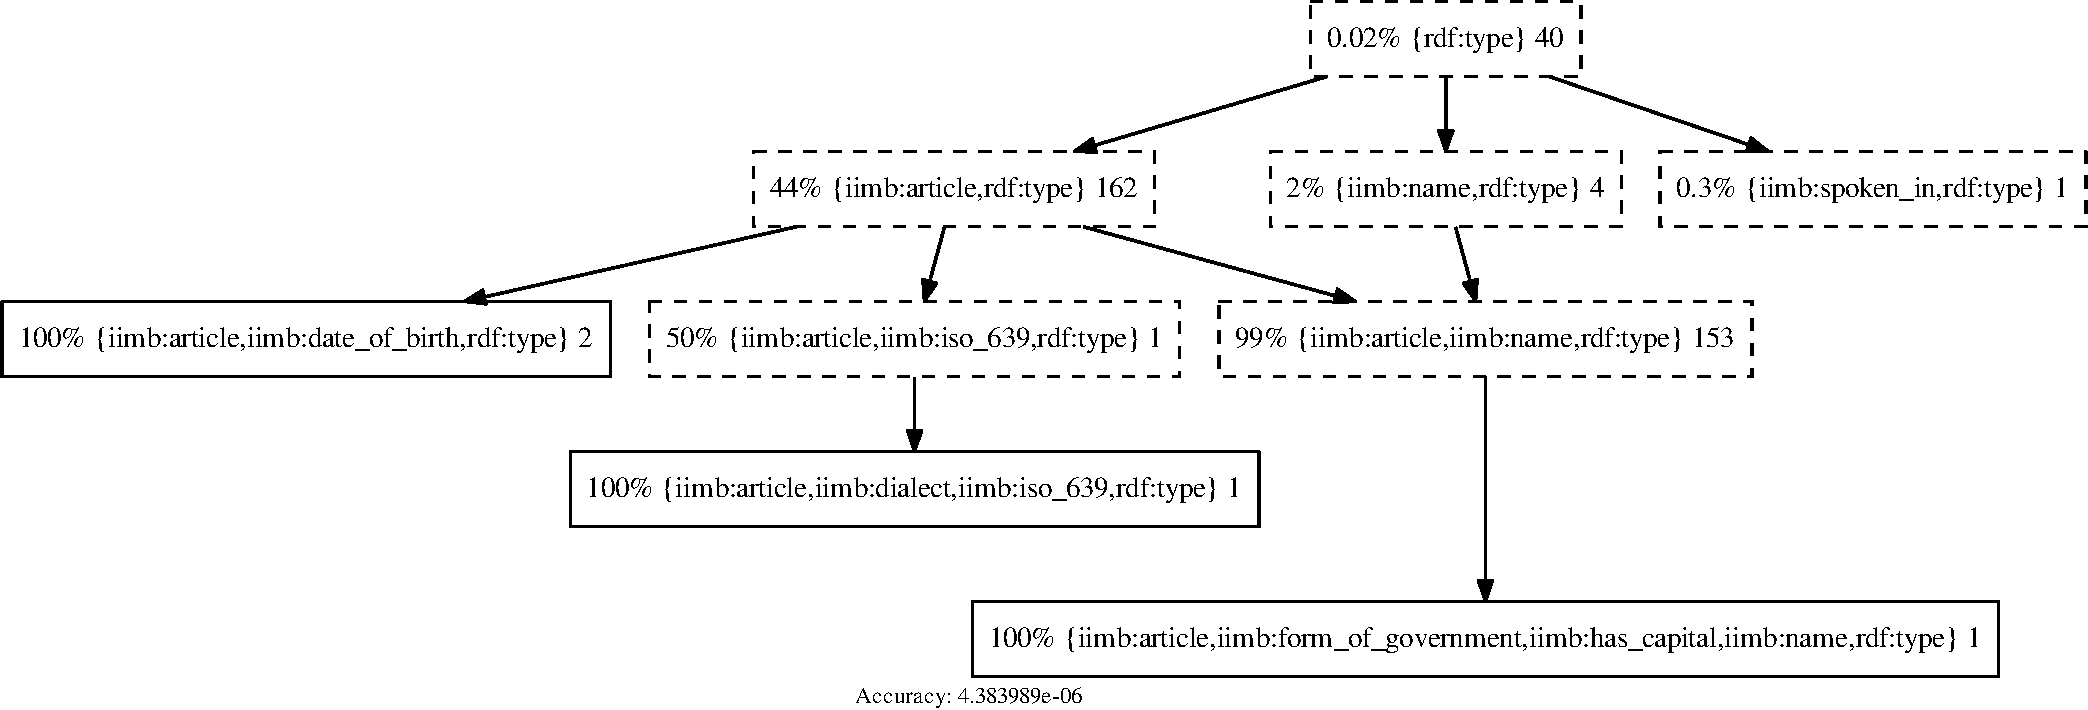
\includegraphics[width=\textwidth]{iimb_approximation_example_crop}
\caption{
  An example of a discernibility partition for an identity relation
    consisting of 365 pairs applied to the fourth IIMB linkset.
  Each node is annotated with the set of predicates $P$ for which
    its pairs are $P$-indiscernible.
  The number of identity pairs within each partition set
    is displayed to the right of the predicate set label.
  Partition sets that contain no identity pair are not show.
  The number that occurs to the left of the predicate label in each node
    indicates how may pairs in that node are identity pairs.
  The lower approximation consists of the nodes with a solid border,
    indicating that they contain only identity pairs.
  The higher approximation consists of all displayed nodes.}
\end{figure*}

\footnote{
  $P$ must be closed under the identity relation, i.e.,
  \begin{equation*}
    cl_{\sim}(P) = \bigcup_{\tuple{\range{p_1}{p_n}} \in P}\nolimits (
      [p_1]_{\sim} \times \ldots \times [p_n]_{\sim}
    )
  \end{equation*}
}
\end{comment}


\subsection{Quality \& Approximation}
\label{sec:approximation}

Not all identity subrelations have the same quality.
Indeed, when we look at the subdivision into three `categories' above,
  we are able to distinguish between a lower approximation of identity,
  as the union of subrelations from the first category
  (definition \ref{def:identity_lower_approximation}),
  and a higher approximation of identity,
  as the union of subrelations from both the first and the second category
  (definition \ref{def:identity_higher_approximation}).

\begin{definition}[Lower approximation]
\label{def:identity_lower_approximation}
\begin{align}
  x \in \lowerapprox
\, \iff \,
    \setdef{y}{x \equiv_{\indp_{\approx}} y}
  \; \subseteq \;
    \approx\nonumber
\end{align}
\end{definition}

\begin{definition}[Higher approximation]
\label{def:identity_higher_approximation}
\begin{align}
  x \in \higherapprox
\, \iff \,
      \setdef{y}{x \equiv_{\indp_{\approx}} y}
    \, \cap \,
      \approx
  \; \neq \;
    \emptyset\nonumber
\end{align}
\end{definition}

\noindent Based on these approximations we can give
  the rough set representation $\pair{\lowerapprox}{\higherapprox}$
  of identity relation $\approx$ \cite{Pawlak1991}.
The quality of a rough set representation is given in
  definition \ref{def:quality}.
The intuition behind this quality measure is that the crispness
  of a set should be proportional to the quality
  of the identity relation on which it is based.
Since a consistently applied identity relation has relatively many
  partition sets that contain either
  no identity pairs (small value for $\lowerapprox$) or
  only identity pairs (large value for $\higherapprox$),
  a more consistent identity relation has a higher accuracy.

\begin{definition}[Quality]
\label{def:quality}
\begin{align}
  \alpha(\approx)
\, = \,
  \dfrac{
    \card{\underline{\sim}}
  }{
    \card{\overline{\sim}}
  }\nonumber
  %\card{\lowerapprox} / \card{\higherapprox}
\end{align}
\end{definition}

\noindent Now that we have a formal metric for quality,
  we can define the characteristics of an ideal identity relation.
Traditionally, the ideal identity relation ensures indiscernibility
  for all expressible properties in the language
  (principle \ref{principle:indiscernibility_of_identicals}).
According to this traditional view, an identity relation becomes of
  higher quality by considering more properties
  according to which two resources are verified to be indiscernible.
We give a different quality criterion by observing that
  for a given identity relation $\approx$,
  defined over a domain of resources $S_G$,
  we can define the notion of full discernibility
  (definition \ref{def:full_discernibility}).

\begin{definition}[Full discernibility]
\label{def:full_discernibility}
A domain $S_G$ is fully discernible with respect to
  a binary relation $\approx$ iff
\[
  \forall x,y \in S_G (
      x \in \equivset{y}
    \lor
      \indp_{\approx}(\equivset{x}) \neq \indp_{\approx}(\equivset{y})
    )
\]
\end{definition}

\noindent From definition \ref{def:full_discernibility}
  it is clear that a domain is fully discernable just in case
  there exists a binary relation $\approx$
  for which \mbox{$\alpha(\approx) = 1.0$}.



